\documentclass[12pt,a4paper,twoside]{article}
\usepackage{fancyhdr}
\usepackage[francais]{babel}
\usepackage[T1]{fontenc}
\usepackage[utf8]{inputenc}
\usepackage{color}
\usepackage {graphicx}
% --- PACKAGES MATHS ---
\usepackage{amsmath}  % Pour les symboles de base
\usepackage{amssymb}  % Pour les ensembles (R, K, etc.)
\usepackage{amsthm}   % Pour les environnements de théorèmes
\usepackage{hyperref}
\newtheorem{theorem}{Théorème}


\begin{document}
\title{
    \noindent
    
\includegraphics[height=3cm]{univ_logo.png}
    \hfill 
    
\includegraphics[height=2cm]{univ_logo_info.png}  \newline  
      \newline
      \newline
    \color{blue}Le Mans Université\color{black} \\
    Licence Informatique 2ème année
    \\Module 174UP02 Rapport de Projet
    \\Titre du projet
    }
\author{Hugues Astier\\Corentin Jammes\\ Thomas Dequirez}
\maketitle
\newpage
\tableofcontents
\newpage

 \textbf{  Résumé :} Ceci est le résumé de notre projet MAZE-SHOOTER. 
    Nous y expliquons comment nous avons développé le labyrinthe...

\section{Introduction}
\emph{Cette introduction présentera le sujet qui sera traité et le travail avec une
présentation du plan adopté}
Ce document présente le projet de jeu XXX réalisé dans le cadre de la for-
mation de L2 informatique de l’université du Mans pendant la période de
janvier à avril 2026. Ce projet a été développé en langage C avec la librairie
SDL\footnote{ajouter tout autre librairie utilisée}. Ce jeu fait ceci cela . . .
Nous présenterons dans une première partie notre jeu , des scénarios d’uti-
lisation et les principales fonctionnalités puis dans une deuxième partie la
gestion du projet ensuite dans une troisième partie les éléments principaux
de conception (algorithmes,structures de données, .....) ensuite nous présen-
terons l’architecture de notre application (structuration du code en fichiers)
enfin nous montrerons les principaux résultats. Enfin nous présenterons en
conclusion les points forts et les limites de notre travail, les écarts entre la
planification prévisionnelle et le déroulement réel de notre projet et les le-
çons tirés de cette expérience. En annexe nous présenterons un exemple de
débogage et des tests ( jeux d’essai et cas de test d’un exemple au moins -
le fichier .c étant dans le git dans un répertoire dédié "test") ....

\section{Partie 1}
Dans cette première partie nous allons présenter .... . La \autoref{fig:toutou}.  illustre
.....
L’instruction \verb|\begin figure [!h]| force l’image à se positionner comme
on le désire. Le positionnement de l’image dépend également de ses dimen-
sions, si elle est située en bas de page, et qu’elle est trop grande, elle va se
positionner sur la page suivante et le texte qui suit se retrouvera donc avant
l’image. Il faudra réduire la taille. Ceci peut se faire avec l’option scale de
includegraphics.

\begin{figure}[h]
    \centering
    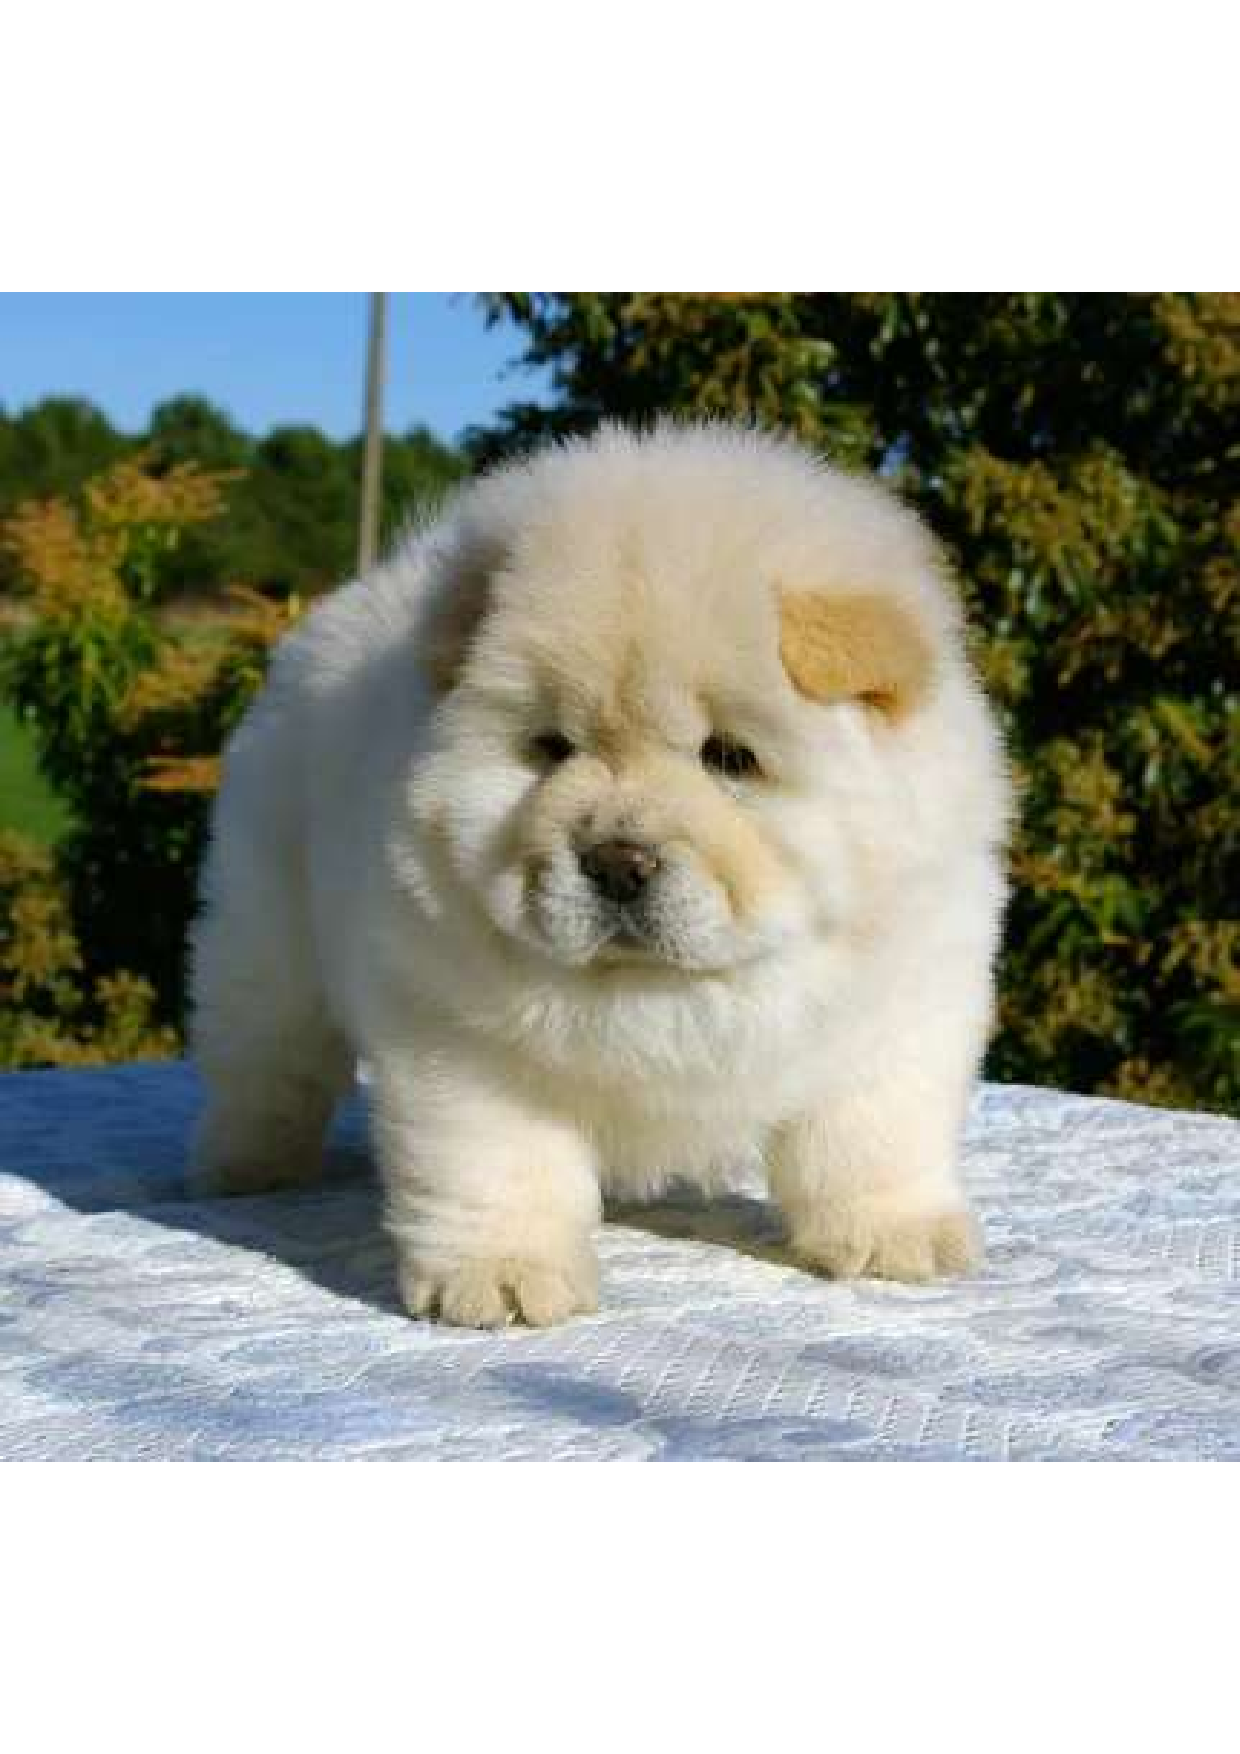
\includegraphics[width=5cm]{chowchow.pdf}
    \caption{Le toutou du projet}
    \label{fig:toutou} 
\end{figure}




  \subsection{Sous titre 1}
  \subsection{Sous titre 2}
\section{Partie 2-Les tableau en Latex}
\section{...}
\section{Bibliographie}
\section{annexe}


\end {document}